\subsubsection*{L'inclinazione del piano}

Se abbiamo capito abbastanza bene il fenomeno dello scivolamento della pila, dovremmo essere in grado di impostare e risolvere un esercizio di questo tipo:\newline

{\bf Testo:}
Un mobile scivola su un piano in clinato con accelerazione costante sia in discesa che in salita, ma in discesa l'accelerazione vale $2.74 m/{s^2*}$, mentre in salita vale $9.02 {m/s}$.

Calcolare l'inclinazione del piano e il coefficiente d'attrito.\newline

{\bf Soluzione}
Il problema può essere rappresentato dalla figura qui sotto, che abbiamo già ossevato in precedenza.

\begin{figure}[H]
 \centering
 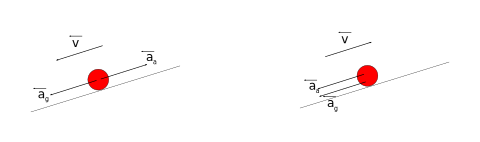
\includegraphics[width=.7\textwidth]{../immagini/leCauseDelMotoDellaPila.png}
 \label{fig:causeDelMotoDellaPila}
\end{figure}

Dai dati del problema definiamo $a_d = 9.02 m/{s^2}$ l'accelerazione totale in discesa e $a_s = - 2.74 m/{s^2}$ quella del moto di salita. Negativa per sottolineare la direzione opposta a quella precedente.

Osservando la figura si può scrivere:
\begin{center}
\begin{equation}
\left\{
\begin{array}{r}
a_s = a_{//} + a_a \\
a_d = a_{//} - a_a
\end{array}
\right.
\end{equation}
\end{center}

In questo sistema, $a_{//}$ e $a_a$ sono due incognite che possono essere risolte sommando e sottraendo membro a membro:\newline

\begin{center}
\begin{math}
\left\{
\begin{array}{r}
a_{//} = \frac{1}{2} a_s + a_d = 5.88 m/{s^2} \\
a_a = \frac{1}{2} a_s - a_d = 3.14 m/{s^2}
\end{array}
\right.
\end{math}
\end{center}

L'accelerazione verso il basso $a_g$ dipende dalla gravità e dall'inclinazione del piano, che può determinata in questo modo:
\newline

\begin{math}
sen \vartheta = \frac{a_{||}}{g} = \frac{5.88\ m/s^2}{9.8\ m/s^2} = 0.60 \\
\end{math}
\begin{math}
\vartheta = arcsen\ 0.60 = 0.64\ rad = 36.9° 
\end{math}

A questo punto è possibile calcolare il coefficiente di attrito. Prima di tutto, dobbiamo cercare l'accelerazione vincolare, che è un cateto del triangolo rettangolo formato con la gravità e l'accelerazione parallela:\newline

\begin{math}
a_{\perp} = \sqrt{g_2 - a_{a}} = \sqrt{9.8^2 - 5.88^2} = 7.84 m/s^2
\end{math}

\begin{math}
\mu = \frac {a_a}{a_\perp} = \frac{3.14}{7.84} = 0.4
\end{math}
